%% Einrichtungen für Beamer-Klasse
\documentclass{beamer}
%\mode<presentation>
%{
%	\usetheme{Warsaw}
%	\usecolortheme{whale}
%	\useinnertheme{rectangles}
%	\usefonttheme{structurebold}
%	\useoutertheme{smoothbars}
%}
%\setbeamercovered{transparent}

% Abschalten der kleinen Navigationsleiste am unteren Rand
%\beamertemplatenavigationsymbolsempty   

% Seitenzahl in Fußnote
%\setbeamertemplate{footline}[frame number] 

% Komisches Einblenden deaktivieren
%\setbeamercovered{invisible}

% KIT-Stil
\usepackage{Stylestuff/beamerthemekit}

%% Deutsche Silbentrennung und Beschriftungen
\usepackage[ngerman]{babel}

%% UTF-8-Encoding
\usepackage[utf8]{inputenc}

%% Bibliotheken für viele mathematische Symbole
\usepackage{amsmath, amsfonts, amssymb}

%% Anzeigetiefe für Inhaltsverzeichnis: 1 Stufe
\setcounter{tocdepth}{1}

%% Schönere Schriften
\usepackage[TS1,T1]{fontenc}

%% Tabellen
\usepackage{array}
\usepackage{multicol}

%% Bibliothek für Graphiken
\usepackage{graphicx}

%% der wird sowieso in jeder Datei gesetzt
%%\graphicspath{{../figures/}}

%% Hyperlinks
\usepackage{hyperref}

\usepackage{lmodern}
\usepackage{colortbl}
\usepackage[absolute,overlay]{textpos}
\usepackage{listings}
\usepackage{forloop}
%\usepackage{algorithmic} % PseudoCode package 

\usepackage{tikz}
\usetikzlibrary{matrix}

%%%%%%%%%%%% INHALT %%%%%%%%%%%%%%%%

%% Wochennummer
\newcounter{weeknum}

%% Titelinformationen
\title[Präsentation zur Implementierungsphase]
%\subtitle{Gehalten in den Tutorien Nr. 1, Nr. 12, Nr. 14 und Nr. 29}
\author[Schmid, Friedmann]{\href{mailto:m-pse@minituex.eu}{Maria Schmid}{\href{mailto:jannis@sycoso.eu}{Jannis Friedmann}} %\href{mailto:dominik.doerner@student.kit.edu}{Dominik Doerner} und \href{mailto:allenouyue@hotmail.com}{Yue Ou}}
\institute{KIT - Karlsruher Institut für Technologie}

%% Titel einfügen
\newcommand{\titleframe}{\frame{\titlepage}}

%% Alles starten mit \starttut{X}
%\newcommand{\starttut}[1]{\part{Tutorium Nr. #1}\setcounter{weeknum}{#1}\titleframe\frame{\frametitle{Inhaltsverzeichnis}\tableofcontents} \AtBeginSection[]{%
\begin{frame}
	\tableofcontents[currentsection]
\end{frame}\addtocounter{framenumber}{-1}}}

%% Kontakt einfügen
\newcommand{\contact}{\begin{center}Kontakt via E-Mail an \href{mailto:m-pse@minituex.eu}{Maria Schmid}\href{mailto:jannis@sycoso.eu}{Jannis Friedmann}} %\href{mailto:dominik.doerner@student.kit.edu}{Dominik Doerner} oder \href{mailto:allenouyue@hotmail.com}{Yue Ou}\end{center}}

%% Letzte Seite mit Bild []
\newcommand{\lastframe}[3]{\part{end}\frame[plain]{\begin{figure}[H]\centering\includegraphics[scale=#1]{#2}\caption{ \url{#3} }\end{figure} \contact}}

%% Frage für Frage und Antwort Spiel
%\newcommand{\frage}[2]{
%\begin{frame}
%	\frametitle{Was bleibt?}
%		\textit{#1}
%		\newline
%		\hspace*{2em} \only<2>{#2}
%\end{frame}		
%}

%% Wörter
\newcommand{\code}[1]{$\mathbf{#1}$}

%% Sterne

\newcounter{starsc}
\newcommand{\stars}[1]{
	\hfill
	\begin{minipage}{100px}
		\forloop{starsc}{0}{\value{starsc} < #1}%
		{%
			\includegraphics[scale=0.05]{star-full.pdf} \hspace*{1px}
		}%
		\forloop{starsc}{\value{starsc}}{\value{starsc} < 5}%
		{%
			\includegraphics[scale=0.05]{star-empty.pdf} \hspace*{1px}
		}
		\vspace*{2px}
	\end{minipage}
}

%% Verbatim
\usepackage{moreverb}


\newcommand{\nM}{\mathbb}
\newcommand{\nR}{\mathbb{R}}
\newcommand{\nN}{\mathbb{N}}
\newcommand{\nZ}{\mathbb{Z}}
\newcommand{\nQ}{\mathbb{Q}}
\newcommand{\nC}{\mathbb{C}}
\newcommand{\nK}{\mathbb{K}}
\newcommand{\nF}{\mathbb{F}}
\newcommand{\nG}{\mathbb{G}}
\newcommand{\nullel}{\mathcal{O}}
\newcommand{\einsel}{\mathds{1}}
\newcommand{\nP}{\mathbb{P}}
\newcommand{\Pot}{\mathcal{P}}

\newcommand{\boder}{\ensuremath{\textcolor{blue}{\vee}}\text{} }
\newcommand{\bund}{\ensuremath{\textcolor{blue}{\wedge}}\text{}}
\newcommand{\bimp}{\ensuremath{\textcolor{blue}{\to}}\text{}}
\newcommand{\bnot}{\ensuremath{\textcolor{blue}{\neg}}\text{}}
\newcommand{\bone}{\ensuremath{\textcolor{blue}{1}}\text{}}
\newcommand{\bzero}{\ensuremath{\textcolor{blue}{0}}\text{}}

\newcommand{\summe}[2]{\sum\limits_{#1}^{#2}}
\newcommand{\limes}[1]{\lim\limits_{#1}}

\newcommand{\numpp}{\advance \value{weeknum} by -2 \theweeknum \advance \value{weeknum} by 2}
\newcommand{\nump}{\advance \value{weeknum} by -1 \theweeknum \advance \value{weeknum} by 1}



\newcounter{abc}
\newenvironment{alist}{
  \begin{list}{(\alph{abc})}{
      \usecounter{abc}\setlength{\leftmargin}{8mm}\setlength{\labelsep}{2mm}
    }
}{\end{list}}

\renewcommand{\mod}{\text{ \bf{mod} }}
\renewcommand{\div}{\text{ \bf{div} }}

\newcommand{\sgn}{\text{sgn}}


\begin{document}

\section{User Interface}
\begin{frame}
	\frametitle{Login}
	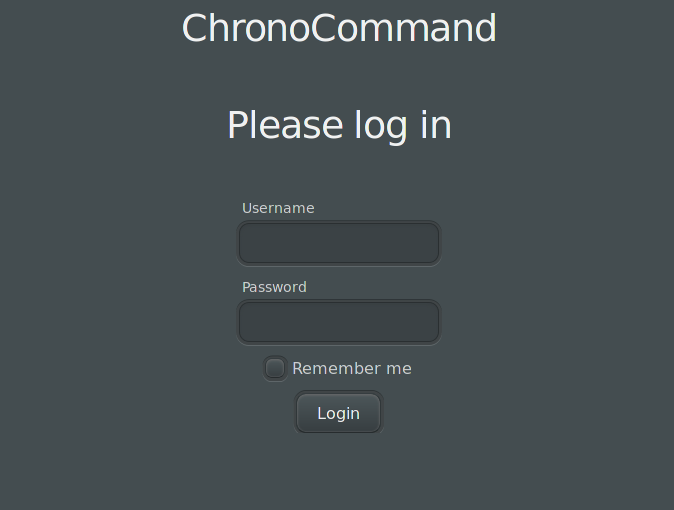
\includegraphics{images/login.png}
\end{frame}

\begin{frame}
	\frametitle{Zeiterfassung bearbeiten}
	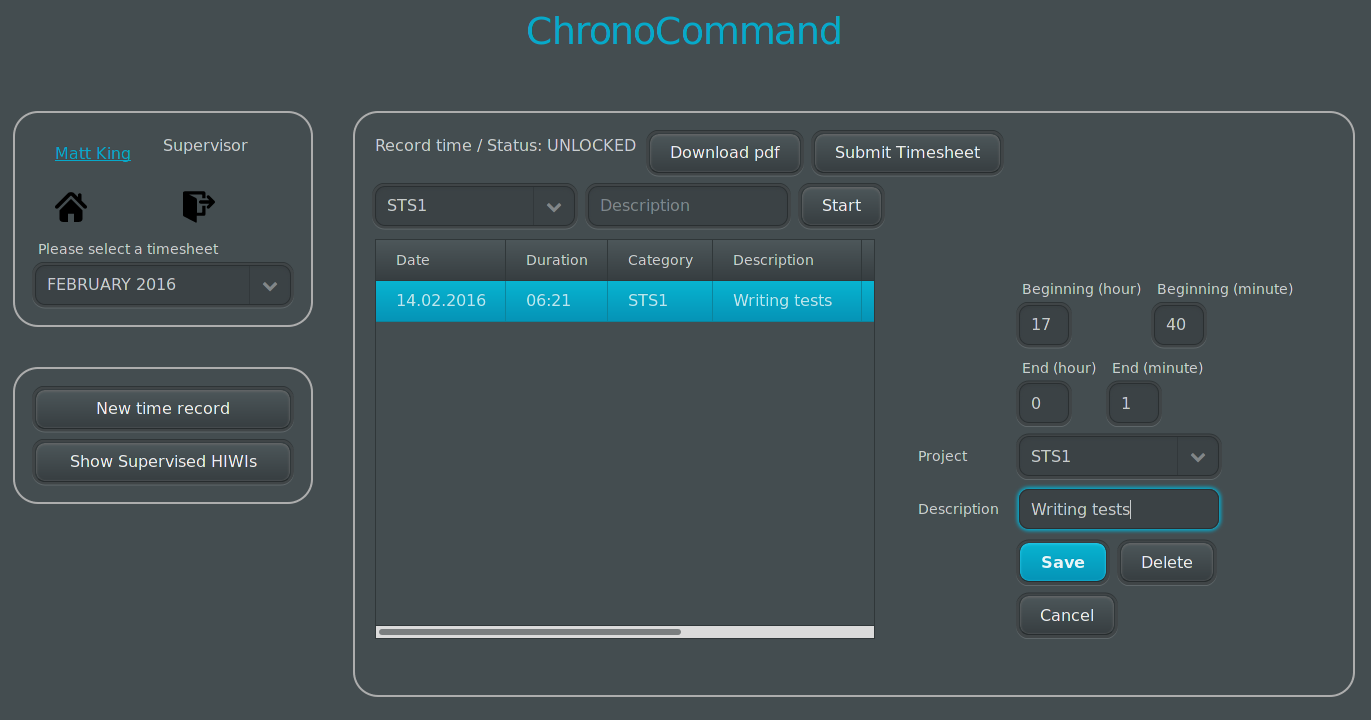
\includegraphics{images/timerecord-edit.png}
\end{frame}

\begin{frame}
	\frametitle{Nutzerübersicht des Administrators}
	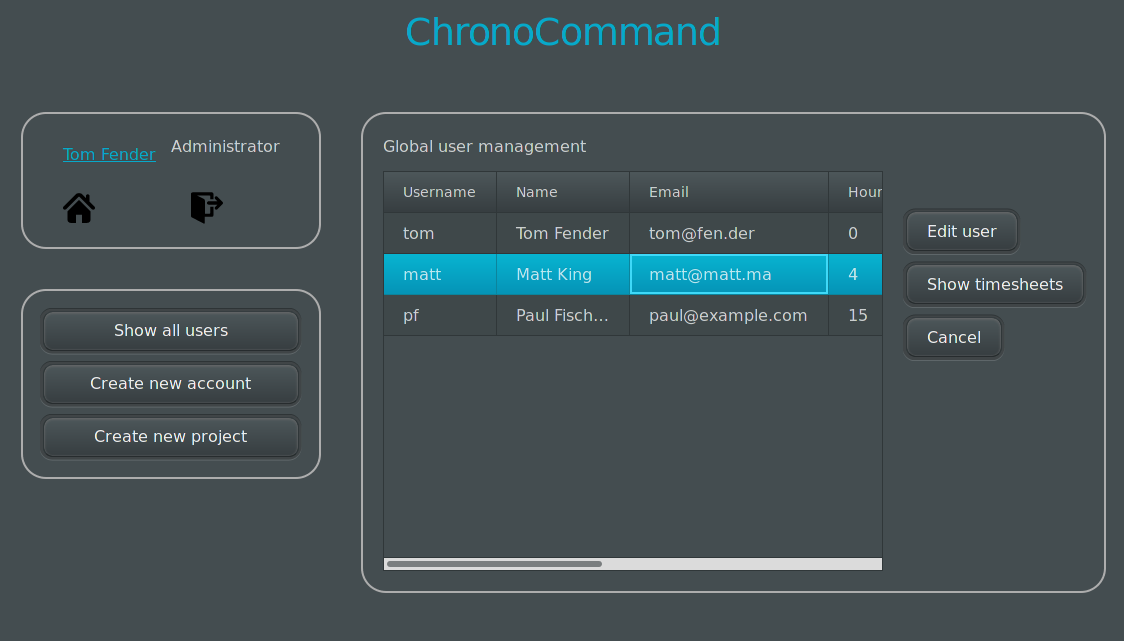
\includegraphics{images/admin-overview.png}
\end{frame}

\begin{frame}
	\frametitle{Neuen Benutzer erstellen}
	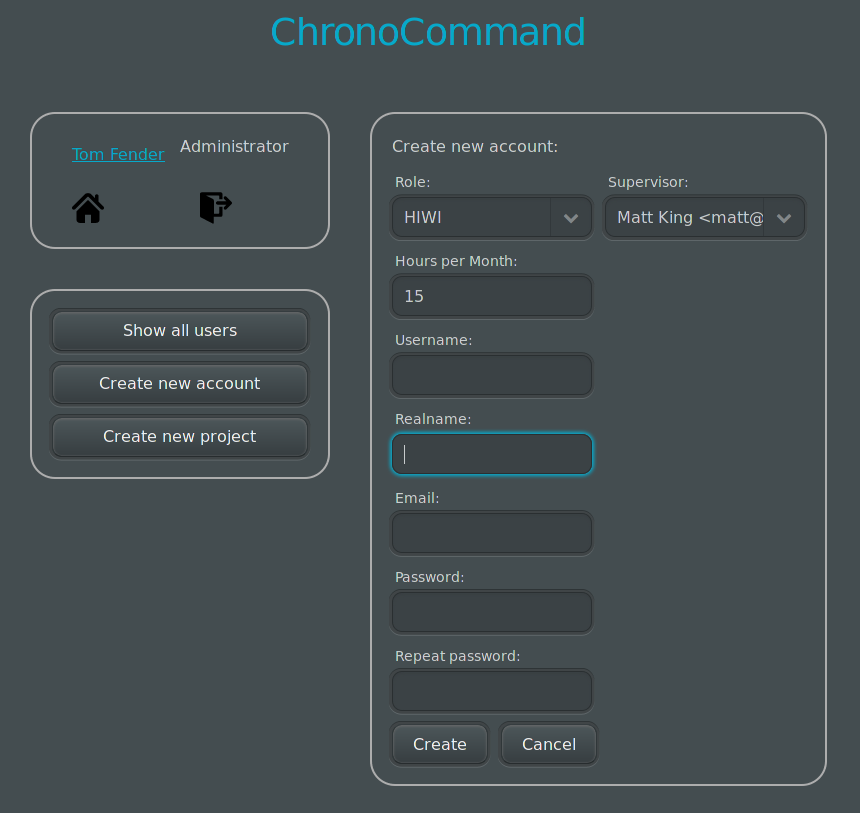
\includegraphics{images/create-user.png}
\end{frame}

\begin{frame}
	\frametitle{Stundenzettelübersicht eines Users}
	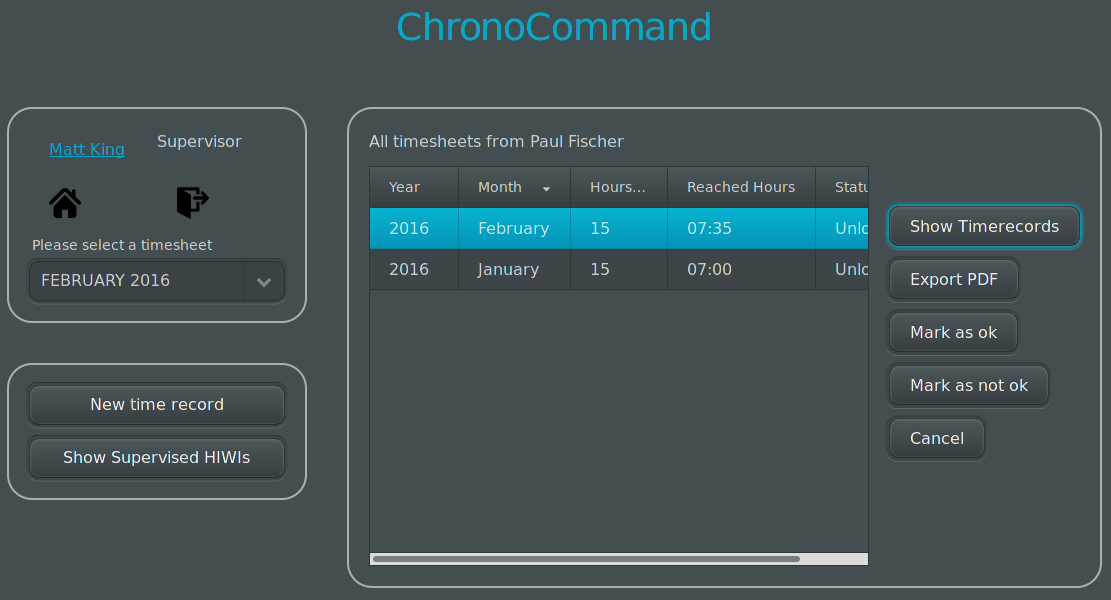
\includegraphics{images/timesheets-overview.png}
\end{frame}


\section{Probleme}

\subsection{Allgemein}
- Unerfahren
- Frameworks nicht genau genug im voraus angeschaut
- In vorherigen Phasen zu ungenau gearbeitet
-> Wasserfallmodell eher shit
- Interne Schnittstellen nicht richtig definiert und kommuniziert

\subsection{Probleme mit Frameworks}

\begin{frame}
	\frametitle{Probleme mit Frameworks}
	
\includegraphics{images/shiro-logo.png}
\end{frame}

\begin{frame}
	\frametitle{Probleme mit Frameworks}
	
\includegraphics{images/hibernate-logo.png}
\end{frame}

\begin{frame}
	\frametitle{Probleme mit Frameworks}
	
\includegraphics{images/vaadin-logo.png}
\end{frame}

% ggf PDFbox
% ggf Quartz


\section{Kriterien}

\subsection{Musskriterien}
% tabelle

\subsection{Wunschkriterien}
% tabelle


\section{Große Veränderungen}


\begin{frame}
	\section{Statistiken}
	\begin{itemize}
		\item Lines of code: 4373
		\item Klassen: 54
		\item Test linecoverage: 21%
		\begin{itemize}
			\item control: 44%
			\item model: 40%
			\item security: 40%
			\item view: 0%
		\end{itemize}
	\end{itemize}
\end{frame}

\end{document}
